\documentclass{article}
\usepackage{relsize}
\usepackage{tikz} % ,pgf,pgfarrows,pgfnodes,pgfautomata,pgfheaps,pgfshade}
\usetikzlibrary{shapes,decorations,shadings,positioning,arrows,snakes,3d}
\usepackage{amsmath,enumerate,xspace,subfig,siunitx}
\tikzstyle{legend} = [red, fill=white, font=\footnotesize, inner sep=2pt, rounded corners=0.05cm]
\tikzstyle{arrow} = [red, ->, line width=2pt]

\usepackage{amsmath,enumerate,xspace,subfig,siunitx,lscape}
\usepackage{listings}
\usepackage[absolute,overlay]{textpos}
\usepackage[colorinlistoftodos]{todonotes}

\usepackage[colorlinks=true,linkcolor=red,pagecolor=red,
  citecolor=blue,urlcolor=blue,breaklinks=true,
  hyperfootnotes=false,pdftitle={CombLayer Guide},
  pdfauthor={Stuart Ansell},pdfkeywords={CombLayer,MCNP,MCNPX}]
           {hyperref}
\renewcommand*{\rmdefault}{cmss}


\definecolor{SlateBlue}{rgb}{0.1,0.1,1.00}
\definecolor{SlateGreen}{rgb}{0.1,0.8,0.3}
\definecolor{darkred}{rgb}{0.8,0,0}
\newcommand{\tcg}[1]{
   \textcolor{green}{#1}}
\newcommand{\tcr}[1]{
   \textcolor{red}{#1}}
\newcommand{\tcb}[1]{
   \textcolor{blue}{#1}}
\newcommand{\tcbb}[1]{
   \textcolor{SlateBlue}{#1}}
\newcommand{\tcgg}[1]{
   \textcolor{SlateGreen}{#1}}


\definecolor{mygray}{rgb}{0.4,0.4,0.4}
\definecolor{mygreen}{rgb}{0,0.8,0.6}
\definecolor{myorange}{rgb}{1.0,0.4,0}

\lstset{
  basicstyle=\small\sffamily\color{black},
  commentstyle=\color{red},
  frame=false,
  numbers=left,
  numbersep=5pt,
  numberstyle=\tiny\color{mygray},
  keywordstyle=\color{blue},
  showspaces=false,
  showstringspaces=false,
  stringstyle=\color{myorange},
  tabsize=8,
  otherkeywords={std},
  escapeinside={\%\%}{\@},
  xleftmargin=0.0\linewidth
}
\newcommand {\prog}[1]{{\it #1}}
\newcommand {\vb}[1]{\begin{\verbatim}{#1}\end{verbatim}}
\newcommand {\alert}[1]{\textcolor{red}{#1}}
\newcommand {\checkme}[1]{\alert{#1}\marginpar{\alert{$\leftarrow$\,check me}}}
\lstnewenvironment{bash}{\lstset{language=bash,numbers=none,backgroundcolor=\color{yellow!20},frame=tb}}{}
\lstnewenvironment{cpp}{\lstset{language=C++,numbers=none,backgroundcolor=\color{green!10},frame=tb}}{}
\lstnewenvironment{deck}{\lstset{language=bash,numbers=none,backgroundcolor=\color{gray!10},frame=tb}}{}
\lstnewenvironment{xml}{\lstset{language=xml,numbers=none,backgroundcolor=\color{green!10},frame=tb}}{}

\setlength{\parindent}{0in}
\setlength{\parskip}{0.1in}
\setlength{\textwidth}{6.5in}
\setlength{\textheight}{9.0in}
\setlength{\oddsidemargin}{0.0in} 
\setlength{\evensidemargin}{0.0in} 

\newcommand{\mcnp}{{\tt MCNP}\xspace}

\newcommand{\figref}[1]{Fig.\,\ref{#1}}
\newcommand{\figrefp}[1]{Fig.\,\ref{#1} on page~\pageref{#1}}


\title{CombLayer Guide}
\author{Stuart Ansell}

\usepackage{nomencl}
\makenomenclature

\begin{document}
\maketitle
\tableofcontents
\clearpage
\printnomenclature[2cm]
\clearpage


\input{Frames/Introduction}
\newpage
\input{Frames/Layout}
\subsection{Expected Component Structure}
\label{Sec:Structure}

\paragraph{Definitions}

A class that builds a placeable object: i.e a FixedComp or
derivative. But not a componsite of objects that have their own
offset/angles, even if they have a commong starting origin.

E.g. if many object could have different placement to each other, then
they are a composite (e.g. a beamline). But an object that has a few
objects within it (for example bolts in a flange) and those included
object don't have a variable modified origin relative to the primary
origin. E.g they don't have a local xStep,yStep etc.


If a class is a placeable object then it should inherrit from
FixedComp directly or via one of the FixedComp derivatives in
attachComp.

It will not inherit from FixedUnit or any of its derivatives.



\paragraph{Object}

The object has to satify a number of abstract virtual methods.

void createAll(Simulation\&,const FixedComp\&,const long int);

This is a public method that builds the object. Typically it will call
in order:

\begin{lstlisting}[language=C++]{Name=MainProg}{floatplacement=H}
  populate(FuncDataBase);
  createUnitVector(FixedComp,const long int);
  createSurfaces();
  createObjects(System);
  createLinks();
\end{lstlisting}

It is strongly discouraged to call any of these sub-methods with
different arguments as normally this breaks the expected inheritance
system. For example, if cutting surfaces are needed e.g. a front/back
cut, then use ExternalCut or FrontBackCut, do not pass an FixedComp
and link point to createSurfaces.


It is also highly likely that for simple FixedComp, FixedRotate, and
FixedOffset objects, createUnitVector can be left out because these
base classes provided methods are acceptable e.g.

FixedComp::createUnitVector sets the Origin and basis set.

FixedOffset::createUnitVector -- applied the pre and post rotations
along with the offset movement set by the variables:

Using preXYAngle,preZAngle,xStep,yStep,zStep,xyAngle,zAngle.

FixedRotate::createUnitVector applies the pre- post rotations along
all three axis


Additional functionality of the reOrientate call is made after
applying the rotations and offset. The function is automatically
applied (if called for) in all of the FixedXXX class.

The reOrientate function moves one axis to a another global axis with
the minimum rotation

Example ess model -- e.g. Vespa/Odin/


\section{Installation}

CombLayer is primarily designed for the Linux platform and requires a
\CC compiler that supports {\CC}11 or later. The code is available at
\href{https://github.com/SAnsell/CombLayer}{https://github.com/SAnsell/CombLayer},
either as a downloadable
\href{https://github.com/SAnsell/CombLayer/archive/master.zip}{zip
  file} or by cloning/pulling the Git repository:
\begin{bash}
  git clone https://github.com/SAnsell/CombLayer.git
\end{bash}

\subsection{Requirments}

CombLayer requires the GNU Scientific
Library~(\href{https://www.gnu.org/software/gsl}{GSL}),
\href{https://www.boost.org}{boost::regex}, as well as the
\href{https://github.com/fmtlib/fmt}{\{fmt\}} and STL libraries
provided by your \CC compiler. The build process is managed with
\href{https://cmake.org}{CMake}, and the class reference documentation
is generated using \href{https://www.doxygen.nl}{Doxygen}.
Both {\tt gcc} and {\tt clang} compilers are supported.

\subsection{Basic build method}

CombLayer can be built either in the source code directory or in a separate build directory. If built in the source directory, the command is

\begin{bash}
  cmake ./
  make
\end{bash}

or for a separate build directory

\begin{bash}
  cmake -B/path/to/buildDirectory -S/path/to/srcDirectory
  make
\end{bash}

This should make a number of executables, e.g. {\tt ess}, {\tt maxiv},
{\tt reactor}, {\tt fullBuild} etc, which can be used to make a model
with commands listed in the {\tt all.sh} script. For instance, the
\begin{bash}
  singleItem --singleItem Octupole AA
\end{bash}
command generates an output file named {\tt AA1.x}, which is an MCNP
model of an octupole magnet. To generate a FLUKA model, add the {\tt
  -fluka} argument, and for PHITS models, use the {\tt -phits}
argument.

\input{Frames/LinkSystem}

\section{Model Runtime control}

C++ programs start from the main() function and in CombLayer the
runtime control has been keep mostly in the main() function. Clearly
that could be further refactored out but CombLayer lacks the
sophisticated top level type abstraction that is required to do this
in a generic way, so copy/pasted structure is used with variance to
the particular model required. The sole advantage of the abscence of a
top level abstraction is that the user is the freedom in writing new objects
which allows other programs to be incorporated by making their main function
a minor function and directly calling.

The structure of two example main()s will be compared from the units
that exist with the stanard CombLayer distribution. That is {\it
bilbau.cxx} and {\it reactor.cxx}. These build the delft reactor model and the
Biblau low energy spallation source.

First part of the code is along list of \#include's. They are the
mainly dependency list of the objects {\it Simulation, weightManager,
and tallySelector.} This can and should be copied at will. Do not
make an file with them all in [see \ref{Sec:IntroInclude}].

At the end of the include section there is typically, one or two model
specific includes. These normally include {\it makeXXX.h} file and
anything that they directly depend on. In the case of bilbau it is just 
{\it makeBib.h} whilst for reactor it is both {\it makeDelft.h} and \prog{ReactorGrid.h}.





Tallies are the fundamental reason for running MCNPX. However, the
manor in which MCNPX specifies tallies is not compatible with a
vairiable defined model because in most cases the required tally is relative 
to an object whose position is unknown. 

This problem has been addressed by allowing most tallies to use the 
FixedComp link system. 

\subsection{Tally System}

The tally system is accessed either by a simple command line menu
system, or via an XML file. The command line help system is very
primative but can remind the user of the bais

\subsection{Point Tally}
\label{PointTally}

Point tallies are fundamentally a 3D vector in space. In CombLayer,
there are three levels of position available: (a) Real MCNP(X) output
position, (b) CombLayer master origin position before master rotation,
and (c) relative position to an object. Both (a) and (c) are well
supported, however, to do option (b) there needs to be some real care
with the layout of the calling sequence in the main() function. The
fullBuild.cxx example is a suitable option to follow, but checking
will be needed.

\subsubsection{Free Point tally}

The simplest way to put a point into CombLayer is to use a free point.
\begin{bash}
./prog -T point free 'Vec3D(300.0,10.0,5.0)' Output
\end{bash}

This creates a point tally at (300,10,5) in the final output using
neutron tallies with the default energy and time binning system.

\subsection{Fluka Tally System}

\subsubsection{Surface Tally}

The fluka surface tally is accessed via -T surface.

The 

%\section{HowTo}
\begin{itemize}
\item Get real surface number by its relative number: SMap.realSurf(divIndex+103) (see createLinks methods)
\end{itemize}

\subsection{How to put one object into another}

Suppose, we are inserting Spoon into Mug.
Mug is made up of N cells. Spoon is made of one contained component with outer surface.
CombLayer provides several methods to put one object into another:

\begin{cpp}{Name=essBuild}{floatplacement=H}
attachSystem::addToInsertForced(System,   *Mug, *Spoon);
attachSystem::addToInsertSurfCtrl(System, *Mug, *Spoon);
attachSystem::addToInsertControl(System,  *Mug, *Spoon);
attachSystem::addToInsertLineCtrl(System, *Mug, *Spoon);
\end{cpp}

\subsubsection{addToInsertForced}

The outer surface of the Spoon is excluded from the HeadRule of every single cell of Mug.
Even if Mug contains cells which do not intersect with Spoon (e.g. its handle, see \figref{fig:forced}).
{\it Forced} means {\it do it and do not think about it}, but at the same time it means that
{\it I have got something wrong somewhere.}  Normally this is that insufficient link points have been added
to the object, or that the object is a set of split (single cell) volumes.  However, there is the additional
problem that the model may not be correctly constructed at this point, so that the other options seem not to work.
This can be checked by adding a
\prog{SimProcess::writeIndexSim(System,"OutputFilename.txt",0);}
in the code just before the call to insertForced. If there are undefined volumes then the model is not in a state that
any of the \prog{addToInsert} algorithms except \prog{addToInsertForced} can be used. 

\begin{figure}
  \centering
  \begin{tikzpicture}
    \drawMug{0}{0}{}
    \drawSpoon{2}{1}{dashed}
  \end{tikzpicture}
  \caption{addToInsertForced: all cells of Spoon are excluded from all cells of Mug including non intersecting cells. In this example, the Spoon is excluded from the Mug handle even though
  they do not intersect.}
  \label{fig:forced}
\end{figure}


\subsubsection{addToInsertSurfCtrl}

The objective of this function is to use the surface intersections between Mug and spoon to determine which 
cells within Mug intersect the ContainedComp of spoon. The process is done on a cell - ContainedComp level. 

The process is as follows:
\begin{enumerate}

\item{Deconvolves both the Spoon's containedComponent boundary into surfaces.}
\item Deconvolves the Mug into surfaces.
\item{Triple Loops over surfaces of both Mug and Spoon}
  \begin{enumerate}
  \item{Calculate intersection of each surface:surface:surface triplet}
  \item{If a point is within CC and the Mug Cells exclude the CC from the
    MCell}
  \end{enumerate}
\end{enumerate}
   
Thus the spoon is inserted only into those cells of Mug which it intersects~(\figref{fig:surfctrl}).

It is not always better to call {\tt addToInsertSurfCtrl} instead of
{\tt addToInsertForced} in cases that if is certain that an
intersection can must take place (particularly if the CC / Inserting
cells have large numbers of surfaces).

{\tt addToInsertSurfCtrl} is a very expensive function to call,
because you have to check all the surface triplets. So, it runs significantly
slower than addToInsertForced, but the geometry will be faster.

\begin{figure}
  \centering
  \subfloat[Cell 3 is excluded from cell 1; cells 2 and 4 not changed]{
    \begin{tikzpicture}
      \drawMug{0}{0}{}
      \drawSpoon{2}{4}{dashed}
      \node[legend] at (2,2) {1};
      \node[legend] at (-1.25,2) {2};

      \node[legend,blue,fill=white] at (2.25,4.5) {3};
      \node[legend,blue,fill=white] at (2.25,6) {4};
    \end{tikzpicture}
  } \quad
  \subfloat[None of the cells are modified]{
    \begin{tikzpicture}
      \drawMug{0}{0}{}
      \drawSpoon{5}{1}{dashed}
      \node[legend] at (2,2) {1};
      \node[legend] at (-1.25,2) {2};

      \node[legend,blue,fill=white] at (5.25,2) {3};
      \node[legend,blue,fill=white] at (5.25,3) {4};
    \end{tikzpicture}
  }
  \caption{addToInsertSurfCtrl: only needed cells are excluded}
  \label{fig:surfctrl}
\end{figure}

The two remaining methods provide similar functionality but with less
computational overhead, however, there are cell constructs which will
cause them to fail.


\subsubsection{addToInsertControl}

It's a very simple method. The link points from Spoon are uses as a test for each of the cells within Mug. 
The method checks if any of these link point fit inside each of the cells of Mug. If it does, then it cuts Spoon from the Mug cell~(\figref{fig:control}).
It is possible to add a vector of link points to check as a parameter to limit the search.

\begin{figure}
  \centering
  \subfloat[Cell 3 is excluded from cell 1 since cell 3 has a link point inside cell 1.
  Cell 4 is excluded from cell 1 since Mug has a link point which is located inside cell 4.
  Cells 2 is not modifed.]{
    \begin{tikzpicture}
      \drawMug{0}{0}{}
      \node[legend] at (2,2) {1};
      \node[legend] at (-1.25,2) {2};
      \draw[red] (2,5) circle (2pt);

      \drawSpoon{1.8}{3}{dashed}
      \node[legend,blue,fill=white] at (2.05,3.5) {3};
      \node[legend,blue,fill=white] at (2.05,5.5) {4};
      \draw[blue] (2.05,3) circle (2pt);
    \end{tikzpicture}
  } \quad
  \subfloat[Intersection is not made because none of the link points are located in another component.
  Geometry is broken. In order to fix it,
  either define more link points or use another volume inclusion method.]{
    \begin{tikzpicture}
      \drawMug{0}{0}{}
      \node[legend] at (2,2) {1};
      \node[legend] at (-1.25,2) {2};
      \draw[red] (-1.53,2) circle (2pt);
      \draw[red] (-1,2) circle (2pt);
      \draw[red] (0,2.5) circle (2pt);

      \drawSpoon{-0.85}{-1}{dashed}
      \node[legend,blue,fill=white] at (-0.6,-0.3) {3};
      \node[legend,blue,fill=white] at (-0.6,3.5) {4};
      \draw[blue] (-0.6,4) circle (2pt);
      \draw[blue] (-0.6,0.5) circle (2pt);
    \end{tikzpicture}
  }
  \caption{addToInsertControl: intersection relies on the link points}
  \label{fig:control}
\end{figure}

\subsubsection{addToInsertLineCtrl}

If  we have a (big) contained component~(Mug) and some (small)
object which clips it~(Spoon) and we are not certain that the link points 
are contained within each Mug cell, then  {\bf addToInsertControl} can not be reliably used.
However, addToInsertLineCtrl adds an additional check to addToInsertControl, because it 
constructs all the connecting lines between the link points, and if the line 
intersects the other cell, an intersection is made~(\figref{fig:linectrl}).

\begin{figure}
  \centering
  \subfloat[Intersection is not made because the line connecting two link points intersects
  cell 4 outside of a cell belonging to the Mug]{
    \begin{tikzpicture}
      \drawMug{0}{0}{}
      \node[legend] at (2,2) {1};
      \node[legend] at (-1.25,2) {2};
      \draw[red] (-1.53,2) circle (2pt);
      \draw[red] (-1,2) circle (2pt);
      \draw[red] (0,2.5) circle (2pt);

      \drawSpoon{-0.85}{-1}{dashed}
      \node[legend,blue,fill=white] at (-0.6,-0.3) {3};
      \node[legend,blue,fill=white] at (-0.7,3.5) {4};

     \draw[olive] (-1.53,2) -- (0,2.5);
    \end{tikzpicture}
  } \quad
  \subfloat[Cell 4 is excluded from cell 2 since at least one line connecting two
link points intersects the Mug handle at a point which is valid within the spoon 
(shown by red filled circles)]{
    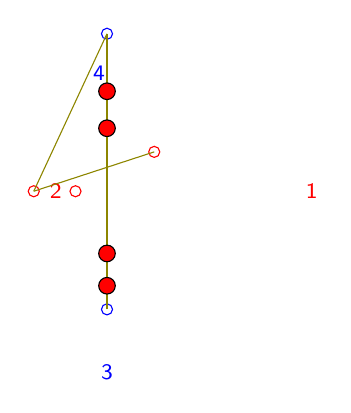
\begin{tikzpicture}
      \drawMug{0}{0}{}
      \node[legend] at (2,2) {1};
      \node[legend] at (-1.25,2) {2};
      \draw[red] (-1.53,2) circle (2pt);
      \draw[red] (-1,2) circle (2pt);
      \draw[red] (0,2.5) circle (2pt);

      \drawSpoon{-0.85}{-1}{dashed}
      \node[legend,blue,fill=white] at (-0.6,-0.3) {3};
      \node[legend,blue,fill=white] at (-0.7,3.5) {4};
      \draw[blue] (-0.6,4) circle (2pt);
      \draw[blue] (-0.6,0.5) circle (2pt);

     \draw[olive] (-0.6,0.5) -- (-0.6,4);
     \draw[olive] (-1.53,2) -- (0,2.5); 

     \draw[olive] (-1.53,2) -- (-0.6,4);

     \draw[fill=red] (-0.6,3.27) circle (3pt);
     \draw[fill=red] (-0.6,2.8) circle (3pt);
     \draw[fill=red] (-0.6,1.21) circle (3pt);
     \draw[fill=red] (-0.6,0.8) circle (3pt);

   \end{tikzpicture}
  }
  \caption{addToInsertLineCtrl: intersection relies on the lines connecting link points (not all link points and connections are shown).}
  \label{fig:linectrl}
\end{figure}


\section{Components}

\input{Components/ObjectRegister}
\input{Components/ExtWeightCommand}

\section{User guide}
This section describes how to use CombLayer from a user's (i.e. non-developer) point of view.
In this guide, it is assumed that the user has no C++ or coding experience.

The guide is focused on the ESS model, which can be generated by running. 
\begin{bash}
  ./ess -r modelOut
\end{bash}
This command produces the \mcnp input file {\tt modelOut1.x} as well as two other files: {\tt ObjectRegister.txt} and {\tt Renumber.txt}.

The single flag {\tt -r} is optional for MCNP6 as it causes the objects and surfaces in MCNP to be renumbered sequentially and
to fit within the 100,000 object/surface limits of MCNPX.

\subsection{Variables}
In the beginning of the input file there is a commented list of variables which define the geometry:

\begin{deck}
 c ----------------------------------------------
 c --------------- VARIABLE CARDS ---------------
 c ----------------------------------------------
 c ABunkerFloorDepth 120
 c ABunkerFloorThick 100
 c ABunkerLeftAngle 0
 c ABunkerLeftPhase -65
 c ABunkerNLayers 1
 ...
\end{deck}

The variable name consists of the component name and its corresponding parameter. For instance,
the first variable {\tt ABunkerFloorDepth} in the list above sets the floor depth of the component called {\tt ABunker}.

Only variables that have needed to be examined are included in this output. Several components are optional and if not built then
their corresponding variables are not seen in the output. All variables start with an initial value and stateless variables are prohibited.
Most variables are defined appropiately within the CombLayer program and obviously can be changed by editing the code and recompiling.
However for a simple variable change that is excessive work so there are a number of methods to change variables from the command line.

\subsubsection{How to change variables}
Any of these variables can be changed either via a command line arguments or an XML file.

As an example, consider changing the Beryllium reflector height.
First of all, we need to find out which variable we need to change and therefore find out the name of the Be reflector
component in CombLayer.

To do this, open the \mcnp geometry and click on any Be reflector cell. Currently, it's cell number 5~(exact number depends on the
CombLayer version you are using).

Now we need to find out which component this cell belongs to.  Find this cell number in the {\tt Renumber.txt} file:
\begin{bash}
grep " 5 " Renumber.txt 
Surf Change:1000006 5                                                           
Cell Changed :1000005 5 Object:BeRef (topBe)       
\end{bash}
It shows that the corresponding Be reflector object is called {\tt BeRef}.

Now we need to find out which {\tt BeRef} variable is responsible for its height:
\begin{bash}
grep BeRef a1.x 
c BeRefHeight 74.2
c BeRefLowRefMat Be5H2O
c BeRefLowWallMat Stainless304
c BeRefRadius 34.3
c BeRefTargSepMat Void
c BeRefTopRefMat Be5H2O
c BeRefTopWallMat Stainless304
c BeRefWallThick 3
c BeRefWallThickLow 0
\end{bash}

We can guess from this list that the variable we need is called {\tt BeRefHeight}.

\paragraph[Command line]{Changing variables via command line}
In order to change a variable via command line arguments, run:
\begin{bash}
  ./ess -r -v BeRefHeight 50 modelOut
\end{bash}
Several variables can be changed, e.g.:
\begin{bash}
  ./ess -r -v BeRefHeight 50 -v BeRefRadius 35 modelOut
\end{bash}

Note that it is possible that you miss spell one of the variables, if this is the case then
you will be presented 

\begin{bash}
./ess -r -v BeRefHHH 1 modelOut
Failure to find variable name BeRefHHH             MainProcess[F]::setRunTimeVariable
Exiting from BeRefHHH not found                    ::main
Exit Stack:                                        ::main
::main                                             ::main
  MainProcess::InputModifications                  ::main
    MainProcess::setVariables                      ::main
      MainProcess[F]::setRunTimeVariable           ::main
\end{bash}

Like most CombLayer error messages it is expected that you read them from top to bottom. So the first thing it tells you is
that variable BeRefHHH does not exist in the model. Second that this is a fatal error and finally the calling stack that generated
that error. If you are not debugging the code etc, then only concern yourself with the error/warning messages above the line {\it Exit Stack:}.


It is also possible to use strings and Vec3D objects as variables:
\begin{bash}
  ./ess -r -v BeRefTopRefMat Nickel \
           -v ABunkerQuakePtA0 'Vec3D(1200,191.2,0.0)' modelOut
\end{bash}

will set the Top reflector material to {\it Nickel} and the start of the dilitation joint at 1200,191.2,0 (relative to
target centre. Note that on bash you will need to hard quote (single quote) the Vec3D value or it will
be split into commands.


\paragraph[XML file]{Changing variables with XML file}
Create an XML file with the following content:

\begin{xml}
<?xml version="1.0" encoding="ISO-8859-1" ?>
<metadata_entry>
  <Variables>
  <variable name="BeRefHeight" type="double">50</variable>
  <variable name="BeRefTopRefMat" type="string">Nickel</variable>
  </Variables>
</metadata_entry>
\end{xml}

and generate the modified geometry:
\begin{bash}
  ./ess -r -x model.xml modelOut
\end{bash}

All the variables can be exported in the XML file by running
\begin{bash}
  ./ess -r -X modelOut.xml modelOut
\end{bash}
Note that the {\tt -X} command will overwrite existing files.

The commands can be done combined simulantiously with both XML and command line and output.
\begin{bash}
  ./ess -r -X modelOut.xml -x model.xml -v BeRefHeight 80.0 modelOut 
\end{bash}

This will first read the model.xml file and change the variables. Second it will
change {\tt BeRefHeight} to 80, and finally write out the XML file of all variables to the file
{\tt modelOut.xml}.

\paragraph[Dependent variables]{Dealing with dependent variables}
If some other variables depend on the variable you are going to change, it can break the geometry.
Consider, for instance, changing the BeRef radius from the baseline value of 34.3 to \SI{40}{\centi\meter}:
\begin{bash}
  ./ess -r modelOut
\end{bash}
this generates the \SI{34.3}{\centi\meter} model\footnote{34.3\,cm is the baseline BeRef radius in the commit {\tt e47bf6d}.} as shown in \figref{fig:user:BeRef:343}.

Now let's set it to \SI{40}{\centi\meter}:
\begin{bash}
  ./ess -r -v BeRefRadius 40 modelOut
\end{bash}
This geometry is shown in \figref{fig:user:BeRef:40:wrong} and it is broken since now {\tt BeRef} intersects with the Bulk component.


\begin{figure}
  \centering
  \subfloat[Baseline radius of \SI{34.3}{\centi\meter} \label{fig:user:BeRef:343}]{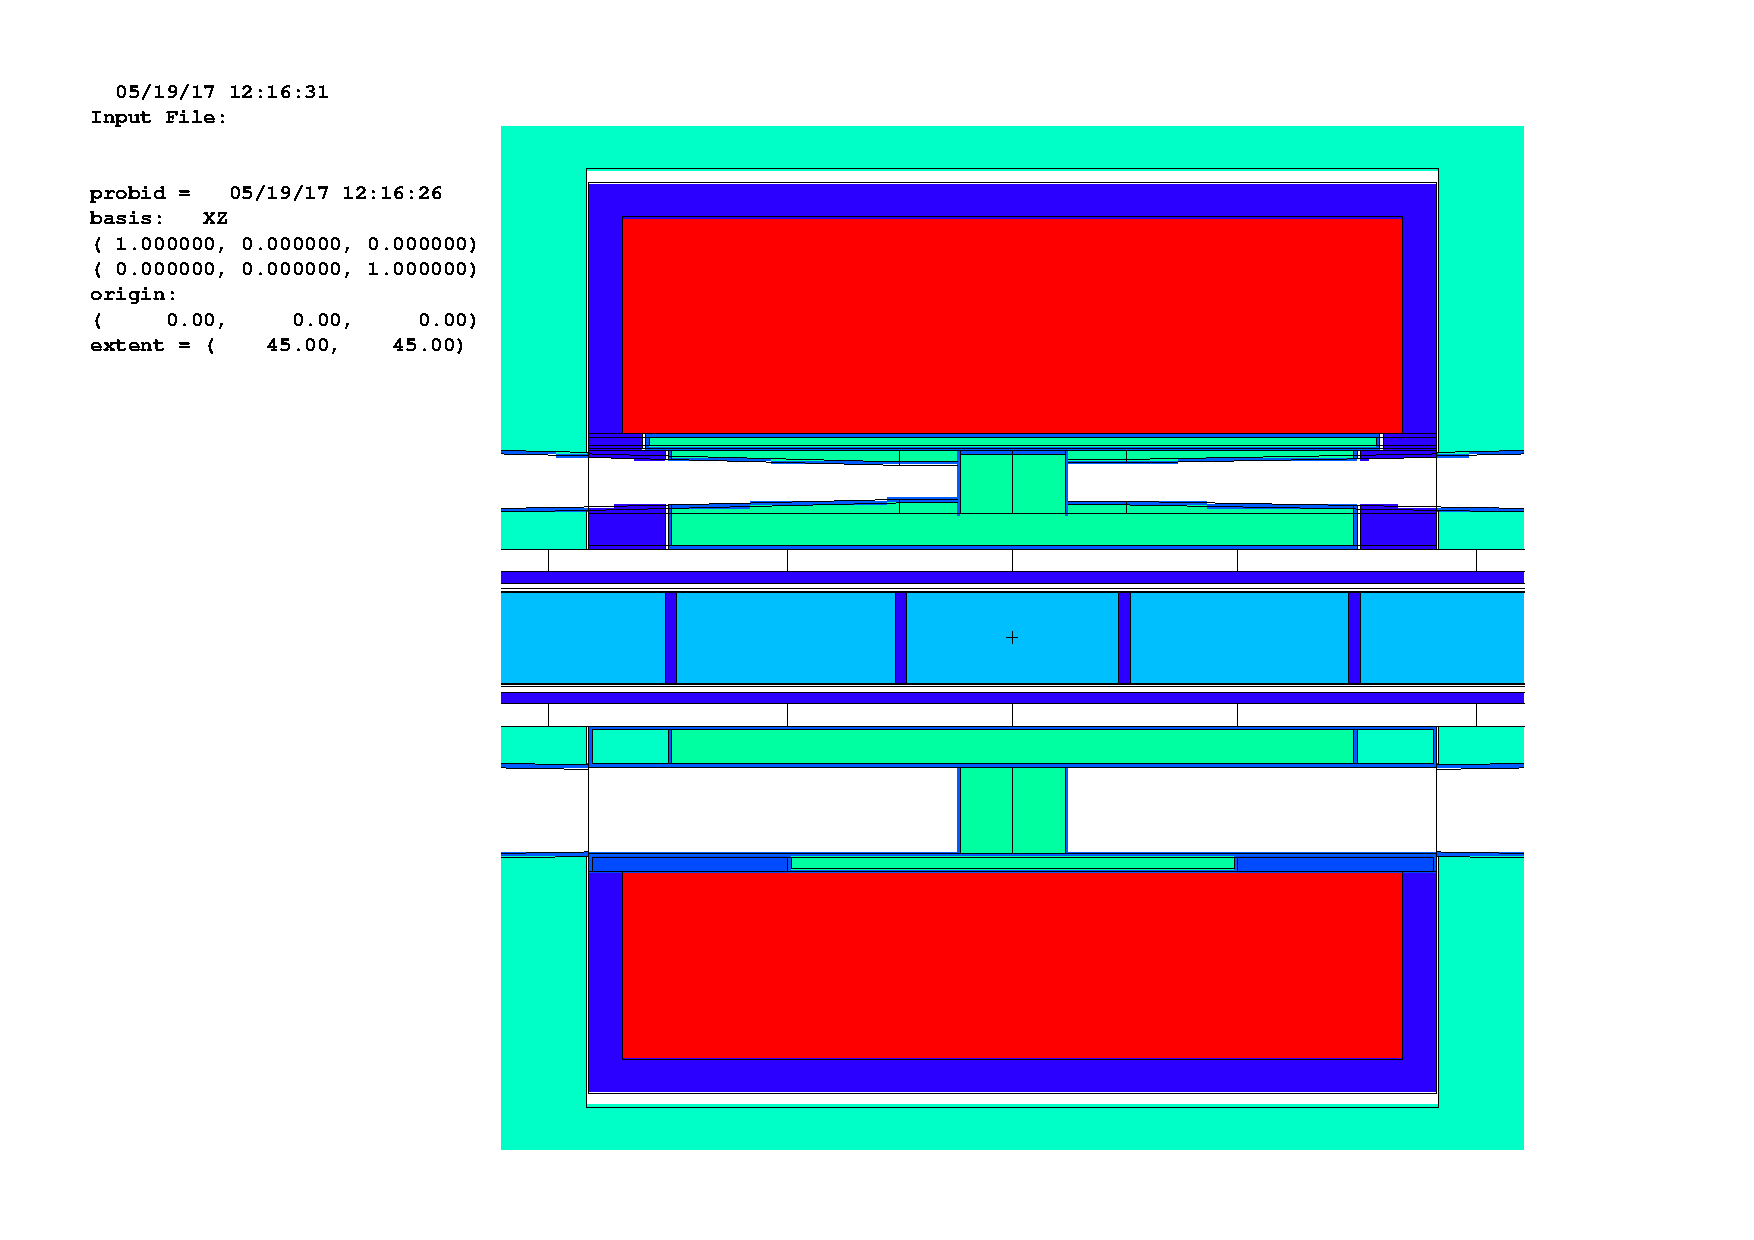
\includegraphics[width=0.5\textwidth, clip=true, trim=8.5cm 10cm 4cm 2.5cm]{UserGuide/BeRefRadius343.pdf}}~
  \subfloat[{\tt BeRefRadius} increased to \SI{40}{\centi\meter} without taking into account dependent variables, which produced geometric errors \label{fig:user:BeRef:40:wrong}]{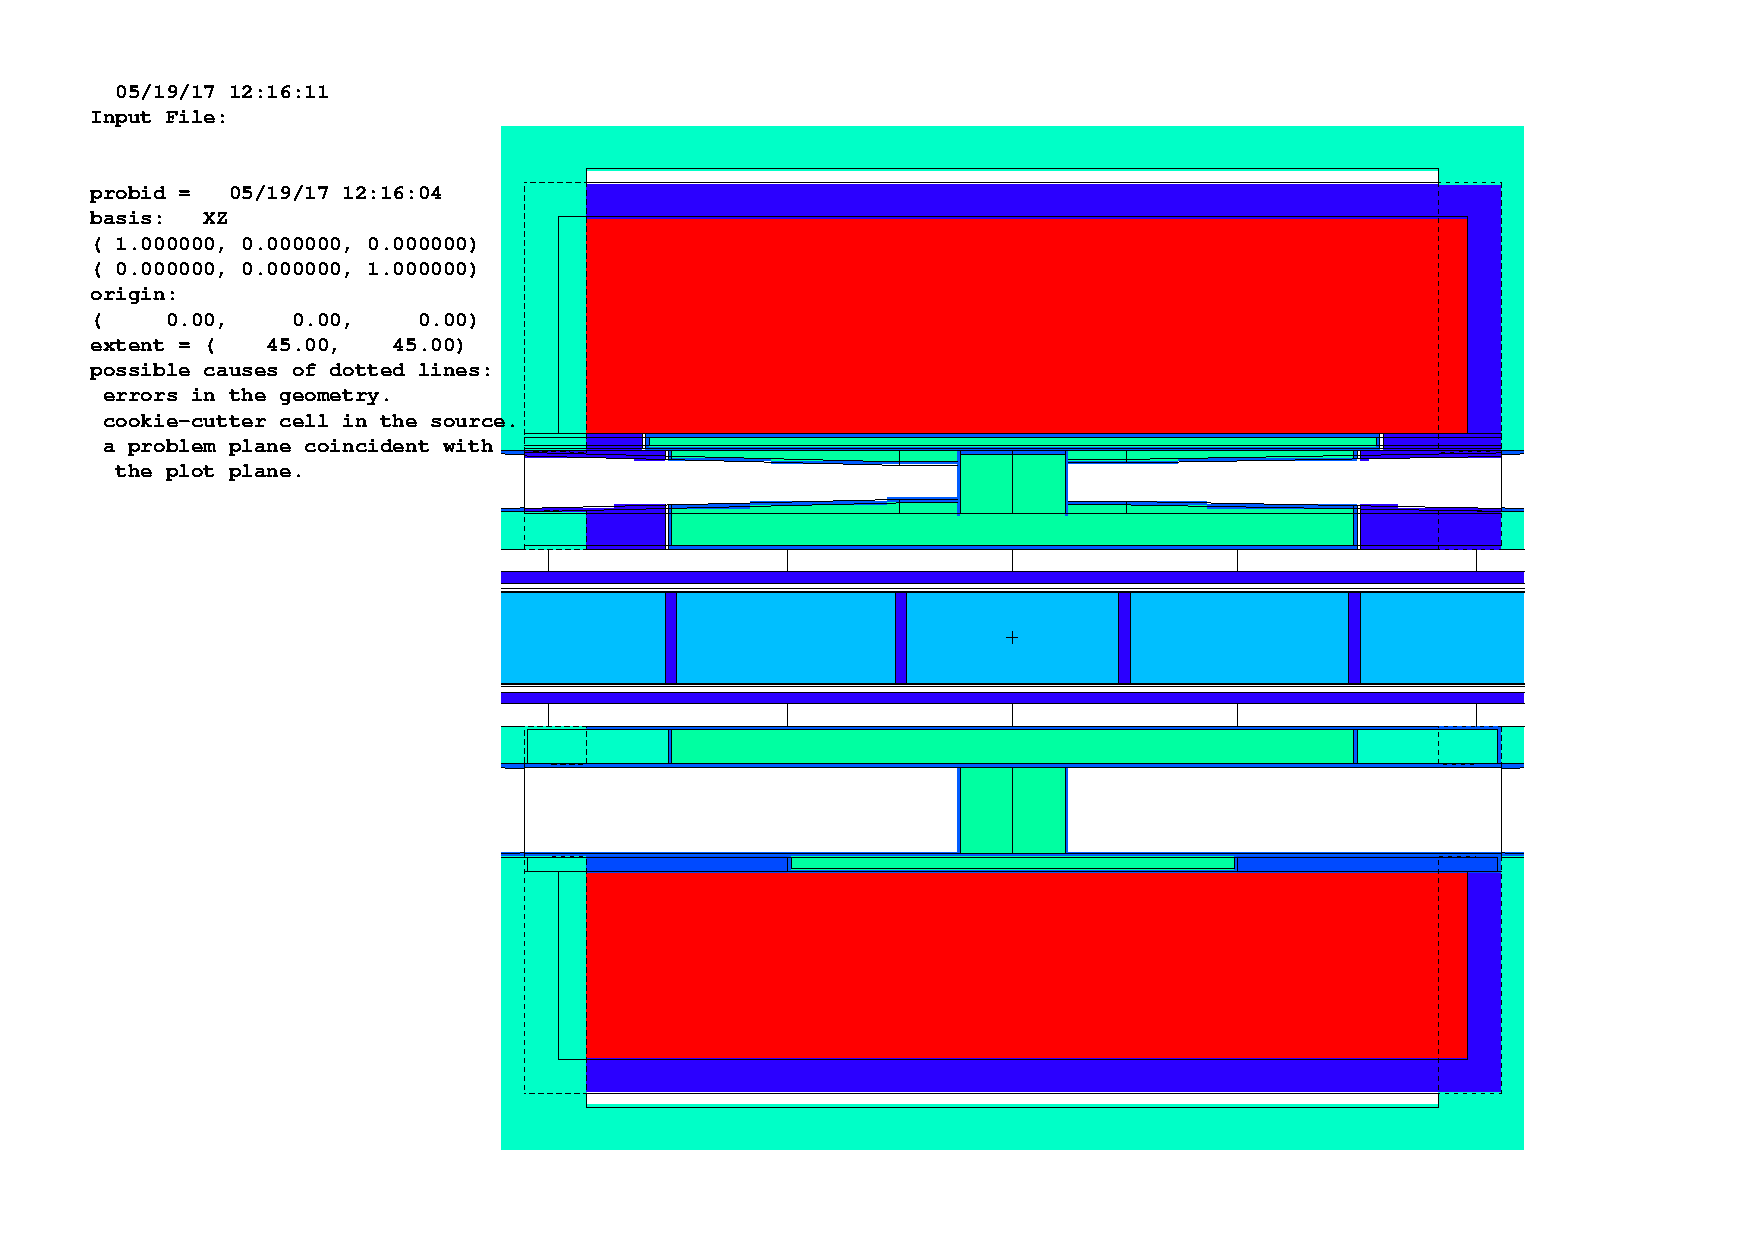
\includegraphics[width=0.5\textwidth, clip=true, trim=8.5cm 10cm 4cm 2.5cm]{UserGuide/BeRefRadius40wrong.pdf}} \\
  \subfloat[{\tt BeRefRadius} increased to \SI{40}{\centi\meter} taking into account dependent variables \label{fig:user:BeRef:40:correct}]{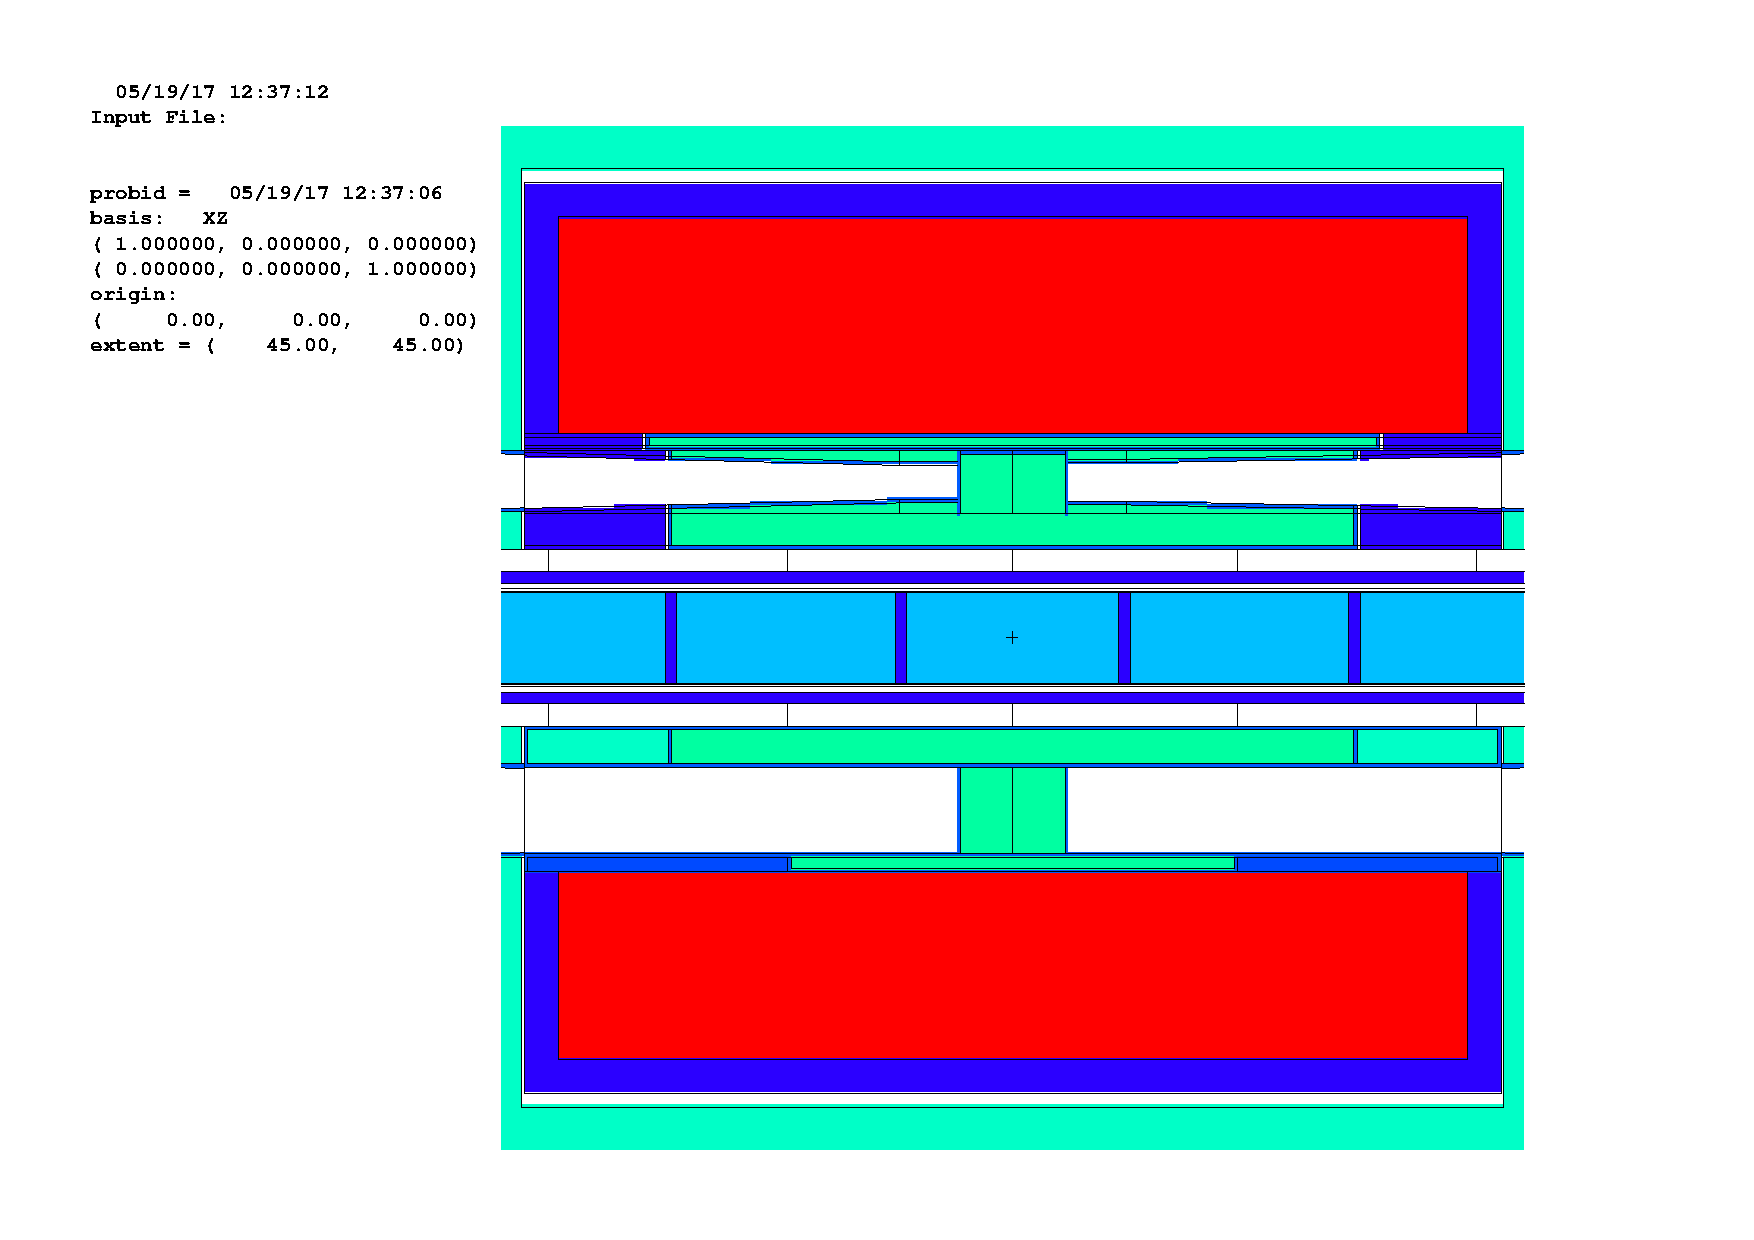
\includegraphics[width=0.5\textwidth, clip=true, trim=8.5cm 10cm 4cm 2.5cm]{UserGuide/BeRefRadius40correct.pdf}}
  \caption{Geometries with different BeRef radii}
  \label{fig:user:BeRef}
\end{figure}

In order to find out which other variables depend on the given one ({\tt BeRefRadius} in our case), find it in the variables setup in the C++ variable definition:

\begin{bash}
 grep BeRefRadius Model/essBuild/*.cxx
 Model/essBuild/essVariables.cxx:  Control.addVariable("BeRefRadius",34.3);
 Model/essBuild/essVariables.cxx:  Control.addParse<double>("BulkRadius1",
                                                   "BeRefRadius+BeRefWallThick+0.2");
\end{bash}
It means that we have to adjust the {\tt BulkRadius1} variable accordingly. This variable depends upon both {\tt BeRefRadius} and {\tt BeRefWallThick}.
Find out the {\tt BeRefWallThick} value:
\begin{bash}
  grep BeRefWallThick modelOut1.x
  c BeRefWallThick 3
\end{bash}
Therefore the {\tt BulkRadius1} value must be $40+3+0.2=43.2$\,cm:
\begin{bash}
 ./ess -r -v BeRefRadius 40 -v BulkRadius1 43.2 modelOut
\end{bash}
which produces the correct geometry shown in \figref{fig:user:BeRef:40:correct}.

\subparagraph{Important note} Sometimes in the C++ variable definitions the dependence is not set explicitly, i.e. in our case {\tt BulkRadius1} would be defined just by the value:
\begin{bash}
 Model/essBuild/essVariables.cxx:  Control.addParse<double>("BulkRadius1",43.2);
\end{bash}
In this case we have to inspect the geometry manually in order to find out which other variables we need to change to produce the correct input deck.

\subsection{Variance reduction}
\subsubsection{Cell-based biasing}
\label{sec:vr:cell}

Cell-based weight window can be generated with the following arguments:

\lstinputlisting[language=bash,numbers=none,backgroundcolor=\color{yellow!20},frame=tb]{UserGuide/cell-biasing.sh}



  The purpose of the variance reduction is to change the weight in the cell by the following equation 
  \begin{equation}
    \label{weigthEqn}
    w_{mod}= \textrm{scaleFactor} \times \frac{\exp (-\sigma \times \rho \times \textrm{densityFactor}
      \times r \times \textrm{rScale}) }
    { (\textrm{rScale} \times r )^{\textrm{r2Power}} }
  \end{equation}

  Note the repeate of rScale in the equation, thus effectively separating densityFactor from rScale.
  For each --weightObject the weight in the cells in modifed by $w_{mod}$ in the equation above 
  
  \begin{description}
\item[-defaultConfig Single ODIN ] These optional arguments build the ODIN beam line
  without building any other beamlines~(see \figref{fig:vr:cell})..

\item[-angle objAxis odinAxis 0] This rotates the model about the 
  master $z$ axis followed by around the master $y$ axis such that
  the FixedComp link-point axis specified after objAxis is collinear with the
  $x$ axis in the final output. In this example the FixedComp is the {\it odinAxis}
  and the link point is zero (which signifies to used the FixedComp origin and Y axis
  rather than a linkPoint).
  This rotation simplifies the weight window source plane setup
  for the current example and used here for illustration purpose.

\item[-w] should precede all weight-related arguments and sets up the model for variance analysis.
  
\item[--weightEnergyType] defines energy grid\footnote{With the {\tt wwg} card you can either use this expression or
  {\tt --wwgE}}.
  The following variants of syntax are possible:
  \begin{enumerate}
    \item If use the word {\em energy} then the format is energy followed by inital weight for that bin
      (in our example: for energies below \SI{0.1}{\mega\electronvolt} the initial weight is \num{0.95};
          for energies between \num{0.1} and \SI{1}{\mega\electronvolt} the initial weight is \num{0.85} etc).
        \item If you drop the word {\em energy} then you just set the energy grid without specifying initial weights
          which are taken to be zero
    \item Alternatively you can use pre-defined keywords:
      {\tt basic}, {\tt high}, {\tt mid} and {\tt flat}\footnote{Energy-weight binnings for these keywords are defined in \tt{System/weights/WeightControl.cxx}}.
  \end{enumerate}
  
\item[--weightSource] This argument defines a point in space.
  We can define as many as we want (by adding several {\tt weightSource} arguments),
  but only those used with {\tt weightObject} will be used. When referenced they will be called S0, S1, S2 ... etc
  based on the order they appear in the command line.
  This particular point is shown by a circle in the left side of \figref{fig:vr:cell:labels}.
  
\item[--weightPlane] This argument defines a plane. Similarly to {\tt weightSource}, we can define as many planes as we want,
  but only those used with {\tt weightObject} will be used.
  When referenced they will be called P0, P1, P2 ... etc based on the order they appear in the command line.
  This particular plane is shown by a dashed vertical line in the right side of \figref{fig:vr:cell:labels}.
  
\item[--weightObject] Define objects we would like to make cell-based variance reduction to.
  \begin{description}
  \item[G2BLineTop20] Object name. It's also possible to specify range of objects within an object or cell name via
    {\tt CellMap}.
  \item[SS0] This is a two part reference. The first letter (S) implies that the item is considered to emmit neutrons.
    The second characters imply that this occurs from the position of the first source point defined above.

  \item[energyCut=0.0] Energy cut. Defines min energy for variance reduction
    (i.e. no modification will occur to energy bins below this value). However, if the number is negative, then
    if defines a -ve maximum energy past which no variance modification will be made.

  \item[scaleFactor=1.0] Linear scale factor in equation \ref{weightEquation}
    It's transport to go from {\em a} cell to another cell.
    \alert{Scale factor is taken out in the mesh based variance reduction because it is identical in effect to the
      command [-wwgNorm scaleFactor 1.0] }

  \item[densityFactor=0.9] Density scale factor. Normally we set it a bit less than one to make it easier to do transport through thick layers
    
  \item[rScale=1.0] Length is adjusted to a different scale effect
    
  \item[r2Pow=2.0] Scale for the length exponent in the distance effect. It should be increased in high absorbing
    regions and decreased in regions that are effectively in a forward going direction for the higher energy scattering
    (effectively mimicking forward angle scattering)
    
  \end{description}

\item[--voidUnMask] The unpopulated world is made of sphere of importance 0 both inside and out.
  All objects that are places in the world must go in the inner spherical volume and they (unless specified) will have
  importance 1.0. In the case that the tally extends into this inner region sphere (e.g. for a dose after a
  shielding wall) must have either (a) a void volume added to the model or (b) the inner part of the world shere set
  to importance zero. This flag does option (b) [This flag may also be used to allow cross talk between two beamlines for
    example] 

\end{description}

\paragraph{Notes}
\begin{itemize}
\item In order to set up biasing, you need at least one source, if you one or more tally (adjoint) points then you must have at least one source.

\item Source can be defined either as a point (via {\bf --weightSource}) or a plane (via {\bf --weightPlane}).
  In the example above we defined point source. However the defined sources and planes do nothing until you use them in
  {\bf --weightObject}.
  
\item General rule to get the things into work: try different setups and compare results. In particular, higher energy
  transport is forward going and it is easy to over weight the splitting when particle would predominately scatter
  in a forward direction. This can be overcome by either reducing the $r^2$ power or decreasing the density.
  Similarly, resonance streaming dominates thick shielding transport but the code does not account for that, so to
  approximate the lower attenuation coefficient the density can be reduced using the density factor. Finally,
  for H$_2$ systems (e.g. polyethelene shielding) the high energy lose term for the hydrogen is not correctly
  weighted (CombLayer uses single group approximation) and additional $r^2$ or Rlength scaling is worth cosidering.

\end{itemize}

% \begin{equation}
%   \label{eq:vr:cellweight}
%   W = \exp{(-w \cdot \sigma_{\text{scale}} \cdot \text{scaleFactor} \cdot \text{factor})}
% \end{equation}

% % CellWeight.cxx
% $$
% factor = minW < \num{1e-16} ? log(\num{1e-16})/log(minW) : 1.0
% $$


\begin{landscape}
\begin{figure}
  \centering
  \subfloat[Horizontal view: geometry \label{fig:vr:cell:labels} ]{
  \begin{tikzpicture}
    \node[anchor=south west,inner sep=0] (image) at (0,0) {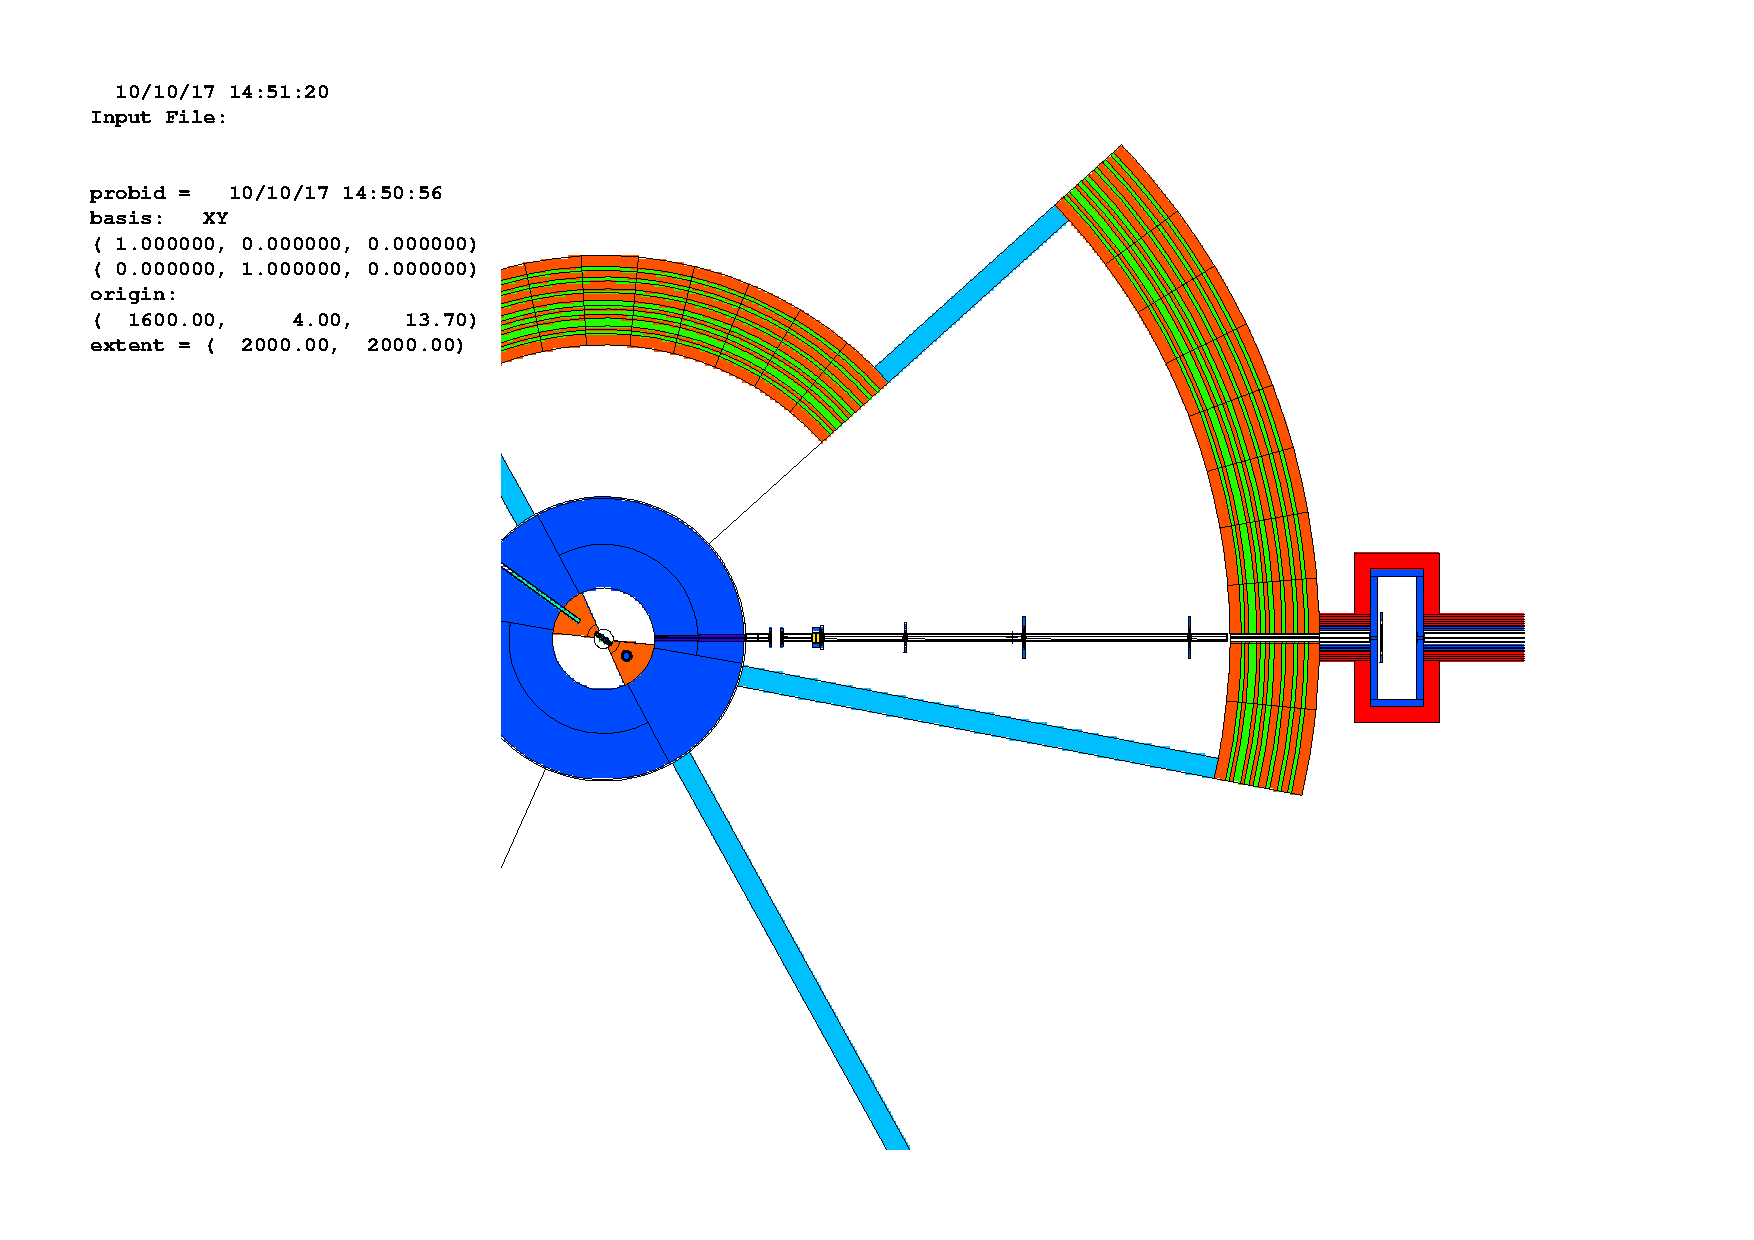
\includegraphics[width=0.5\linewidth,page=1,clip=true, trim=10cm 8cm 4cm 7cm]{UserGuide/cell-biasing.pdf}};
    \begin{scope}[x={(image.south east)},y={(image.north west)}]
      % \draw[help lines, xstep=.1, ystep=.1] (0,0) grid (1,1);
      % \foreach \x in {0,1,...,9} {\node [anchor=north] at (\x/10, 0) {0.\x}; }
      % \foreach \y in {0,1,...,9} {\node [anchor=east]  at (0, \y/10) {0.\y}; }

      \draw[red,thick] (0.07, 0.367) circle (0.5mm);
      \draw[arrow] (0.11,0.46) -- (0.077,0.38);
      \node[legend, anchor=west] at (0.1,0.5) {weightSource};

      \draw[red,dashed] (0.79,0) -- (0.79,1);
      \draw[arrow] (0.85,0.8) -- (0.79,0.8);
      \node[legend, anchor=west] at (0.85,0.8) {weightPlane};

      \draw[arrow]     (0.14,0.2) -- (0.14,0.36);
      \node[legend] at (0.14,0.2) {G2BLineTop20};

      \draw[arrow]                 (0.65,0.25) -- (0.69,0.25);
      \node[legend,anchor=east] at (0.65,0.25) {CBunkerWallMainWall1};

      \draw[arrow]                 (0.65,0.45) -- (0.69,0.45);
      \node[legend,anchor=east] at (0.65,0.45) {CBunkerWallMainWall2};
    \end{scope}
  \end{tikzpicture}
  }
  \subfloat[Horizontal view: wwn]{
    \includegraphics[width=0.5\linewidth,page=2,clip=true, trim=10cm 8cm 4cm 7cm]{UserGuide/cell-biasing.pdf}
  } \\
  \subfloat[Vertical view: geometry]{
    \includegraphics[width=0.5\linewidth,page=3,clip=true, trim=10cm 8cm 4cm 7cm]{UserGuide/cell-biasing.pdf}
  }
  \subfloat[Vertical view: wwn]{
    \includegraphics[width=0.5\linewidth,page=4,clip=true, trim=10cm 8cm 4cm 7cm]{UserGuide/cell-biasing.pdf}
  }
  \caption{Cell-based weight window}
  \label{fig:vr:cell}
\end{figure}
\end{landscape}

\clearpage

\bibliographystyle{unsrt}
\bibliography{Guide}

\end{document}
